%!TEX root = ../thesis.tex


本章では，報酬関数の変化が歩行動作へ与える影響を調査するために行う実験について述べる．
まず，学習に使用したシミュレータや実験を行う環境モデル，エージェントについて述べる．なお，本実験ではNVIDIA Isaac Labで標準提供されているUnitree G1の学習環境（locomotion）を用いる．次に，状態，行動空間や報酬関数について述べる．

\section{実験装置}
本実験の環境を表に示す．
\begin{table}[hbtp]
  \caption{Experimental Setup}
  \label{table:data_type}
  \centering
  \begin{tabular}{lcr}
    \hline
    OS & Ubuntu 22.04 \\
    Simulator  & NVIDIA Isaac Sim \\
    Framework  & NVIDIA Isaac Lab \\
    CPU & Intel ® CoreTM i7-14700 \\
    GPU & NVIDIA GeForce RTX 4090 SUPER \\
    RAM & 32 {GB} \\
    Storage & 2.0 {TB} \\
    \hline
  \end{tabular}
\end{table}


\begin{table}[htbp]
    \centering
    \caption{Actuator Parameters of the Unitree G1 Robot Model}
    \label{tab:g1_actuator_params}
    \small % 表全体の文字サイズを少し小さくする
    % X は幅に合わせて自動調整・折り返しを行う列指定子
    \begin{tabularx}{\linewidth}{Xcccc}
        \toprule
        \textbf{Joint Name} & \textbf{Max Trq.} & \textbf{Max Vel.} & \textbf{Stiffness} & \textbf{Damping} \\
         & [Nm] & [rad/s] & ($K_p$) & ($K_d$) \\
        \midrule
        Hip (Yaw, Roll) & 300.0 & 23.0 & 150.0 & 5.0 \\
        Hip (Pitch), Knee, Torso & 300.0 & 23.0 & 200.0 & 5.0 \\
        Ankle (Pitch, Roll) & 20.0 & 9.0 & 20.0 & 2.0 \\
        Arms (Shoulder, Elbow, Wrist) & 300.0 & 23.0 & 40.0 & 10.0 \\
        \bottomrule
    \end{tabularx}
\end{table}

\begin{table}[htbp]
    \centering
    \caption{Actuator Parameters of the Unitree G1 Robot Model}
    \label{tab:g1_actuator_params}
    % \resizebox{幅}{高さ}{内容} -> 高さを!にすると比率維持
    \resizebox{\linewidth}{!}{
        \begin{tabular}{|l|c|c|c|c|}
            \hline
            \textbf{Joint Name} & \textbf{Max Torque} & \textbf{Max Velocity} & \textbf{Stiffness ($K_p$)} & \textbf{Damping ($K_d$)} \\
             & [Nm] & [rad/s] & [Nm/rad] & [Nms/rad] \\
            \hline
            Hip (Yaw, Roll) & 300.0 & 23.0 & 150.0 & 5.0 \\
            \hline
            Hip (Pitch), Knee, Torso & 300.0 & 23.0 & 200.0 & 5.0 \\
            \hline
            Ankle (Pitch, Roll) & 20.0 & 9.0 & 20.0 & 2.0 \\
            \hline
            Arms (Shoulder, Elbow, Wrist) & 300.0 & 23.0 & 40.0 & 10.0 \\
            \hline
        \end{tabular}
    }
\end{table}

\section{エージェントと環境モデル}
本研究では，エージェントとしてNVIDIA Isaac Labにて標準提供されているUnitree G1のロボットモデルを使用する．
また，実験を行う環境モデルについては，\ref{fig:Environments based on legged locomotion tasks}に示すように，平地環境と不整地環境があり，
不整地環境はピラミッド上の階段，スロープ，凹凸の地面がある．

\begin{figure}[H]
  \centering
  \begin{subfigure}{0.48\columnwidth}
    \centering
    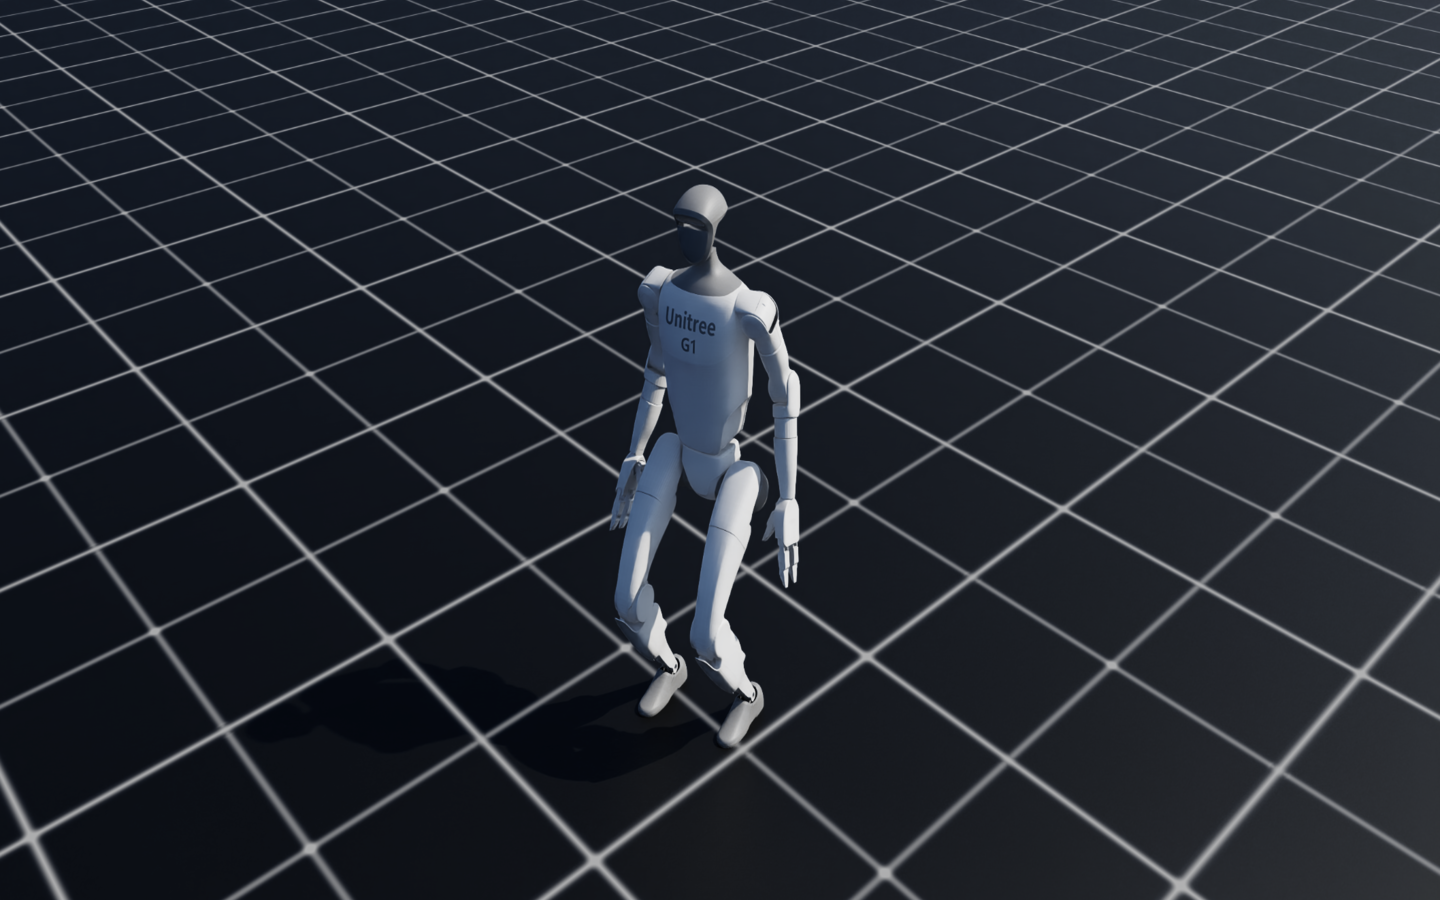
\includegraphics[width=1.0\columnwidth]{images/png/g1_flat.png}
    \caption{Track a velocity command on flat terrain with the Unitree G1}
    \label{fig:velocityflat}
  \end{subfigure}
  \hfill
  \begin{subfigure}{0.48\columnwidth}
    \centering
    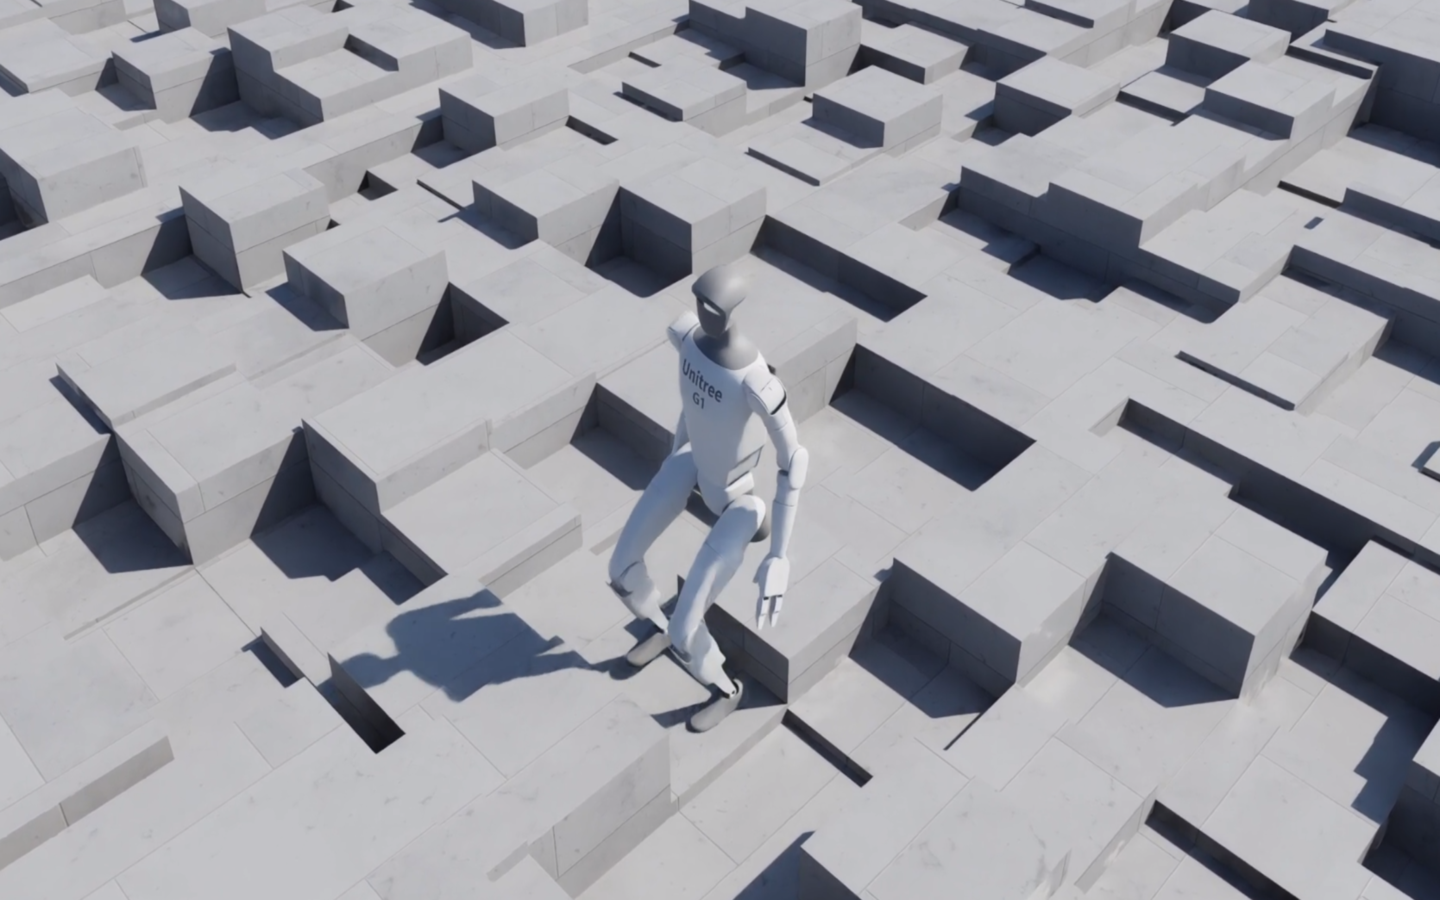
\includegraphics[width=1.0\columnwidth]{images/png/g1_rough.png}
    \caption{Track a velocity command on rough terrain with the Unitree G1}
    \label{fig:velocityrough}
  \end{subfigure}
  \caption{Environments based on legged locomotion tasks}
  \label{fig:Environments based on legged locomotion tasks}
\end{figure}



\section{状態・行動空間}
\subsection{行動空間}
行動空間は，ロボットの各関節に対する目標角度司令で構成される連続空間である．制御周期ごとに，ポリシーネットワークから出力された行動
は，初期姿勢からの相対的な変位として解釈され，スケール係数(0.5)が乗じられた後，デフォルトの関節角度に加算される．
最終的なトルク司令は，Pゲイン(剛性)$K_{p}$およびDゲイン(減衰)$K_{d}$を用いたPD制御則により算出される．

\begin{equation}
  \tau = K_{p}(q_{target} - q) - K_{d}\dot{q}
\end{equation}
ここで，$q$および$\dot{q}$は現在の関節角度および角速度である．

\subsection{状態空間}
表を作る

\section{学習におけるランダム要素}



\section{報酬関数（報酬項）}
本研究では，NVIDIA Isaac Lab，locomotion（二足歩行ロボットが歩行動作＝タスク）を用いる．
本研究における報酬関数は以下の通りである．\par

\begin{itemize}
 \item $R_{termination\_penalty}$ : ロボットが転倒などの致命的な失敗によりエピソードを終了した場合に，学習がそのような状態を避けるよう促すためである．これは，エージェントに対してこの状態に陥ると大きな大きな不利益があることを学習させ，転倒を避ける動作を促す．
 \par
  \begin{equation}
    r_{term} = w_{term} \cdot \mathbb{1}_{terminated}
  \end{equation}
% 指示関数の定義を含む詳細な記述例
ここで，$w_{term} = -200.0$ はペナルティの重み係数であり，$\mathbb{1}_{terminated}$ はエピソードの異常終了を判定する指示関数である．本モデルにおいて，この項はロボットの胴体（torso\_link）が地面に接触した瞬間に適用され，エージェントに対して転倒を回避する強力なバイアスを与える役割を果たす．
  
 \item $R_{track\_lin\_vel\_xy\_exp}$（XY線形速度追従） : エージェントのヨー軸（向いている方向）を基準としたXY平面での線形速度が，目標速度にどれくらい近いか評価し，誤差が小さいほど高い報酬を与える．誤差の評価には指数カーネル（共分散）が使用される．
 \par
 $r_{\text{track\_lin}} = \exp\left(-\frac{\|\mathbf{v}_{xy}^{\text{cmd}} - \mathbf{v}_{xy}^{\text{base\_yaw}}\|_2^2}{\sigma^2}\right)$
 \item $R_{track\_ang\_vel\_z\_exp}$（Z軸角速度追従） : エージェントの目標角速度にどれだけ近いかを評価する．
 \par
 $r_{\text{track\_ang}} = \exp\left(-\frac{(\omega_z^{\text{cmd}} - \omega_z^{\text{world}})^2}{\sigma^2}\right)$

 \item $R_{feet\_air\_time}$（足の滞空時間） : 足が地面から離れている時間（滞空時間）が一定の閾値（）を超えた場合に報酬を与える．これにより，足を地面に擦るのではなく，持ち上げて歩行する動作を促す．
 \par
 $r_{\text{air\_time}} = \max(0, \min(T_{\text{air}, L}, T_{\text{air}, R}) - T_{\text{thresh}})$
 \item $R_{feet\_slide}$（足の滑りペナルティ） : 足が地面に接地していると判定されている間に，その足がワールド座標系のXY方向に速度を持つ（＝滑っている）ことに対してペナルティを与える．
 \par
 $r_{\text{slide}} = \sum_{f \in \{\text{left, right}\}} \|\mathbf{v}_{xy}^{\text{foot}, f}\|_2 \cdot \mathbb{I}(F_{\text{contact}, f} > F_{\text{thresh}})$
 \item $R_{flat\_orientation\_l2}$（水平姿勢維持ペナルティ） : エージェントの胴体が水平から傾くことに対してペナルティを与える．
 \par
 $r_{\text{orientation}} = \| \mathbf{g}_{\text{proj}, xy}^{\text{base}} \|_2^2 = (g_x^{\text{base}})^2 + (g_y^{\text{base}})^2$
 \item $R_{dof\_pos\_limits}$（関節可動域ペナルティ） : 関節角度が設定された可動域の上限または下限に近づくことに対してペナルティを与える．
 \par
 \item $R_{joint\_deviation\_...}$（デフォルト姿勢からの逸脱ペナルティ） : 
 \par
 \item $R_{action\_rate\_l2}$ : 
 \par
 $r_{\text{action\_rate}} = \| \mathbf{a}_t - \mathbf{a}_{t-1} \|_2^2$
 \item $R_{dof\_acc\_l2}$ : 
 \par
 \item $R_{dof\_torques\_l2}$ : 
 \par
 $r_{\text{torque}} = \| \mathbf{\tau} \|_2^2 = \sum_{j \in \text{joints}} \tau_j^2$
\end{itemize}


\newpage
